\subsection{Example Based Super Resolution}
\noindent
Como puede observarse la interpolación soluciona parcialmente el problema de
\emph{Súper Resolución}, pero tiene como consecuencia los efectos mencionados. En
particular, el desenfoque resulta contraproducente al intentar mejorar los 
detalles de una imagen. Por lo mismo, en los algoritmos clásicos de \emph{Súper Resolución}
se utiliza la interpolación únicamente para aumentar la densidad de los pixeles
y aproximar la imagen de salida como una imagen más grande con un determinado 
factor de escalado, pero con los detalles de desenfoque que producen los 
algoritmos de interpolación no adaptativos. 

Para solucionarlo, algunos autores proponen realizar un postprocesado a la imagen 
interpolada para incluir los detalles faltantes y con ello mejorar visiblemente 
la calidad de los bordes de la imagen. 

En particular, \cite{freeman} propone un parchado de la imagen reescalada a partir
de un conjunto de entrenamiento o diccionario de parches en pares de alta
y baja resolución. Dichos parches permiten construir una imagen con frecuencias
altas que no están en la imagen de entrada con el objetivo de sumar la imagen
original interpolada con las frecuencias altas que buscan mejorar su resolución
al realzar sus detalles. En la Figura \ref{fig:fr_algoritmo} puede observarse de
manera específica el algoritmo propuesto basado en el parchado de la imagen de 
entrada mediante un algoritmo de predicción.

\begin{figure}[H]
    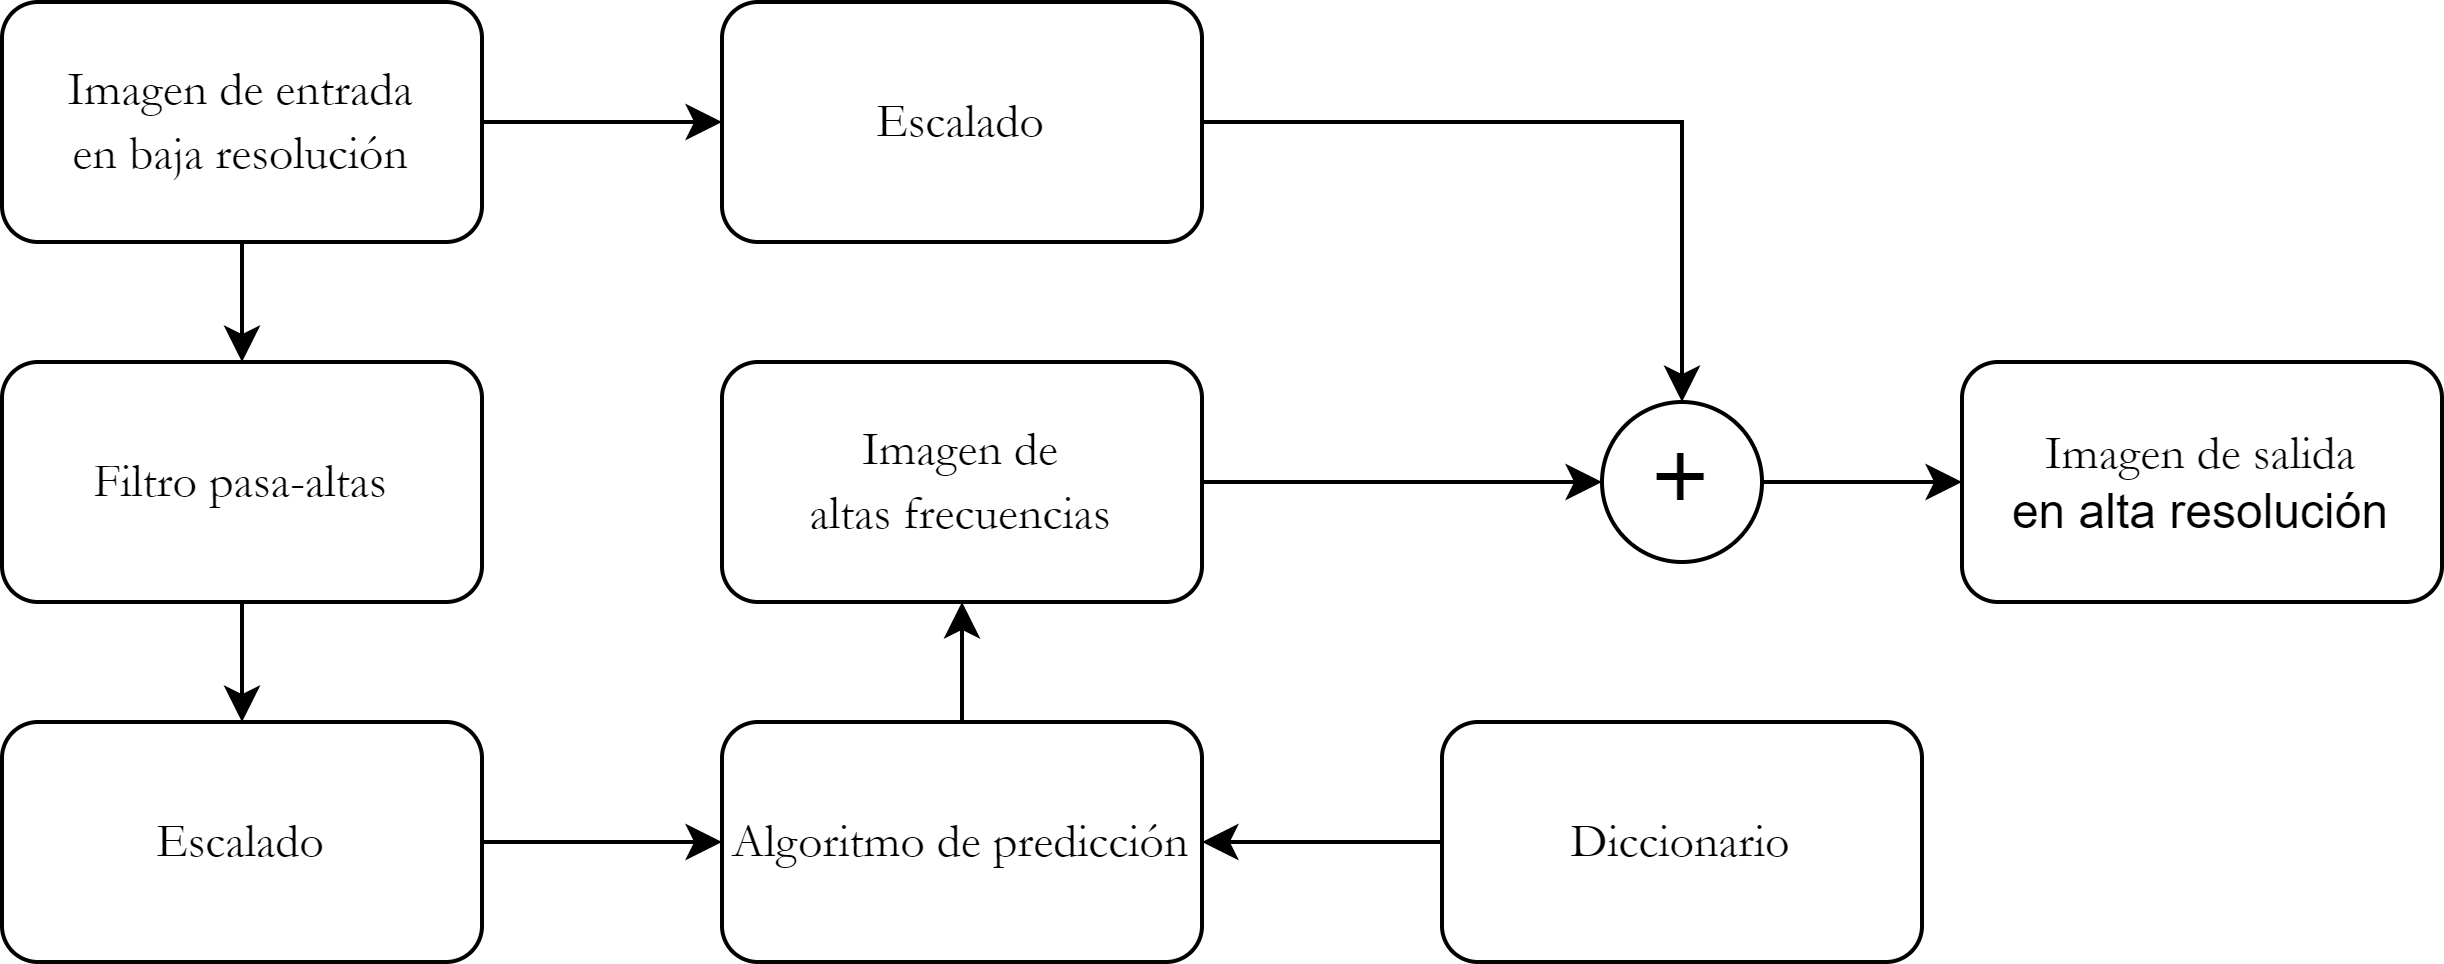
\includegraphics[scale = 0.8]{ fr_algoritmo.png }
    \centering
    \caption{ Algoritmo de súper resolución }
    \label{fig:fr_algoritmo}
\end{figure}

\subsubsection{Diccionario}
\noindent
El algoritmo de \emph{Súper Resolución} \cite{freeman}
opera bajo la premisa que la relación
de predicción entre los parches de alta y baja calidad es independiente del 
contraste de la imagen. Esto también resulta ventajoso, ya que el diccionario 
no necesita ser de imágenes similares a las que se van a reconstruir para 
mejorar la calidad de resolución tal como comenta \cite{diccionario_shuji}.
Esto resulta en un algoritmo general aplicable a cualquier tipo de imagen
y escalable respecto al tamaño de la base de entrenamiento.

Desde el punto de vista de almacenamiento, los parches de baja resolución carecen 
de detalle y por lo tanto predominan las frecuencias bajas, las cuales son 
irrelevantes en su uso para la predicción de detalles y por lo tanto resulta
información necesaria dentro del proceso. Por lo mismo, es aconsejable aplicar un filtro pasa-altas a cada parche 
con el objetivo de dejar sólo la información útil para el algoritmo (detalles).

Por otra parte, para que el diccionario sea funcional sin importar el 
tipo de imagen a reconstruir, se busca normalizar cada pareja de parche con el 
objetivo de mantener su relación intrínseca. De acuerdo con \cite{freeman}, 
los parches de baja resolución se recomiendan con un tamaño de 7x7 pixeles
mientras que los de alta calidad serán de 5x5 todos con centro en el mismo pixel
para mantener la relación. Cabe destacar que la base de entrenamiento está en 
RGB por lo que bastará con el procedimiento antes mencionado para guardar
los pares de parches en algún archivo de fácil acceso. 

\subsubsection{Algoritmo de predicción}
\noindent
Una vez teniendo el diccionario o base de entrenamiento donde se tendrá 
toda la información del algoritmo es necesario establecer el algoritmo de 
predicción para generar esos detalles no visibles en la imagen original.

Para ello, es necesario pre-procesar la imagen de entrada (en baja resolución)
mediante un filtrado pasa-altas para eliminar información innecesaria y posteriormente se realiza
un proceso de escalado mediante algún algoritmo de interpolación para
aumentar sus dimensiones y con ello la densidad de los pixeles tal como se presenta
en la Figura \ref{fig:fr_algoritmo}. Observe que para ese punto, la imagen de entrada
ya sólo cuenta con los pixeles que representan sus bordes o detalles que han sido
escalados con el objetivo de tener una base a partir de la cual se va a reconstruir
con más detalle la imagen de salida. 